\documentclass[journal]{IEEEtran}
\usepackage{amsmath}
\usepackage{amssymb}
\usepackage{algorithmic}
\usepackage{algorithm}
\usepackage{array}
\usepackage{booktabs}
\usepackage{cite}
\usepackage{flushend}
\usepackage{graphicx}
\usepackage{listings}
\usepackage{multirow}
\usepackage{pgfplots}
\usepackage{stmaryrd}
\usepackage{tabularx}
\usepackage{tikz}
\usetikzlibrary{positioning}
\usepackage{url}
\usepackage{verbatim}
\pgfplotsset{compat=1.18}
\usepackage{hyperref}

\begin{document}
\setlength{\tabcolsep}{1pt}
\setlength{\baselineskip}{9pt}
\setlength{\textfloatsep}{3pt}
\setlength{\floatsep}{1pt}
\setlength{\intextsep}{1pt}

\title{Frequency Injection Attacks on SM4 Masking: From RO Entropy to CPA via Second-Order Countermeasures}

\author{Haibo Yi%
        \thanks{Manuscript received November 1, 2026.}\\
        ORCID: \url{https://orcid.org/0000-0002-1635-3738}\\
        \thanks{School of Artificial Intelligence, Shenzhen Polytechnic University, Shenzhen, China. (Email: haiboyi@szpu.edu.cn.) This work was supported in part by Shenzhen Polytechnic University Research Project under Grant No. 6026310054K.}
        }

\maketitle

\begin{IEEEbiography}[{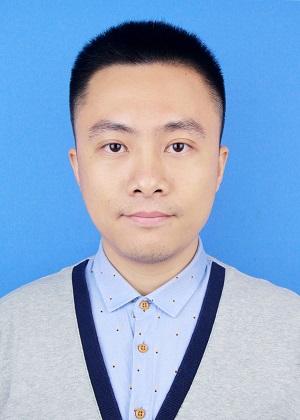
\includegraphics[width=1.25cm]{figures/author_photo.jpg}}]{Haibo Yi}
received the B.S. degree in computer science from Beijing Jiaotong University, Beijing, China, in 2009, and the Ph.D. degree in information security from South China University of Technology, Guangzhou, China, in 2015. He is currently a Professor at the School of Artificial Intelligence, Shenzhen Polytechnic University, Shenzhen, China. His research interests include cryptographic hardware security, side-channel analysis, and FPGA-based cryptographic implementations.
\end{IEEEbiography}

\begin{abstract}
Masking is a cornerstone countermeasure against side-channel attacks, yet its security critically depends on mask unpredictability. This paper quantifies the complete chain from frequency injection attack on the RO-TRNG entropy source through mask degradation to correlation power analysis key recovery, using an FPGA implementation of the Chinese national standard SM4 block cipher as a vehicle. We build an end-to-end simulation platform integrating a gate-level ring oscillator model, statistical entropy evaluation, mask degradation modeling, and security assessment. The key finding is that mask residual strength decays as a sharp threshold function of attacker mask knowledge: only approximately five percent knowledge transitions the attack from total failure to full recovery, stable under measurement noise. We identify a second-order leakage channel in the shared-mask output re-masking engine and propose a byte-wise independent output masking scheme that eliminates this leakage at minimal hardware cost, confirmed by formal verification. The integrated coprocessor is implemented on a commercial FPGA; the SM4 masking engine achieves competitive throughput efficiency, while the RO-TRNG raw output passes the majority of statistical tests and the DRBG post-processed output passes nearly all evaluable tests. This paper provides simulation-based quantitative evidence that RO-TRNG robustness is a necessary condition for masking security.
\end{abstract}

\begin{IEEEkeywords}
SM4, side-channel attacks, masking, frequency injection, RO-TRNG, second-order leakage, FPGA, threshold implementation, min-entropy, AIS-31, formal verification.
\end{IEEEkeywords}

\section{Introduction}

SM4 is the Chinese national cryptographic standard~\cite{gmT0002-2012}, widely deployed in WLAN, mobile communications, and IoT applications. Masking is among the most effective countermeasures against side-channel analysis (SCA), but its security rests on a fundamental premise: masks must be unpredictable. If masks become predictable---for instance, due to physical entropy source interference---the entire masking scheme's security collapses~\cite{wei2024unbalanced}. Frequency injection (FI) is a physical-layer attack against RO-TRNGs: the attacker injects a sinusoidal disturbance into the ring oscillator's power supply line, forcing the RO into a non-ideal oscillation state and degrading output entropy~\cite{sun2023frequency}. Existing work has studied these two aspects---masking cryptography and TRNG robustness---along separate tracks, lacking a systematic analysis that connects them. In this paper, we take an FPGA implementation of the SM4 block cipher as a vehicle and quantify the complete chain from FI-induced RO-TRNG entropy source degradation through mask predictability to CPA key recovery.

\subsection{Background and Motivation}

Frequency injection attacks target RO-TRNG physical entropy sources: when the injected frequency approaches the RO's natural frequency, the RO becomes frequency-locked and its output becomes deterministic~\cite{sun2023frequency}. The literature has explored two independent directions: (1)~\textbf{masking cryptography}, which assumes perfect randomness and studies $d$-order resistance with minimal random bit consumption (e.g., Wei et al.'s unbalanced sharing TI at 2.0 kGE, 8 bits/S-box~\cite{wei2024unbalanced}; Hu et al.'s tower-field CoTG second-order TI at 66 bit/round~\cite{hu2025second}); (2)~\textbf{TRNG robustness}, which studies RO entropy degradation under frequency injection via SP 800-22 tests~\cite{nist2010sp80022,chen2024robustness}. However, few works have connected the two: if the RO entropy source degrades due to frequency injection and masks become predictable, how many CPA traces are needed to recover the key? The answer directly determines the practical security boundary of masking schemes under physical attack, but current understanding remains qualitative rather than quantitative.

\subsection{Contributions}

To address this gap, the main contributions of this paper are:

\begin{enumerate}
\item \textbf{Full-chain integration on a single FPGA bitstream.} The SM4 masking engine, RO-TRNG entropy source, and SP 800-90B health monitoring are integrated into one xc7a200tsbg484-2 bitstream (20,270 LUTs, 15.06\%), with five modules interconnected via AXI-Lite/AXI-Stream---full-chain evaluation from entropy generation to host-level key recovery on a commodity FPGA.
\item \textbf{Byte-wise independent output masking.} Replacing the shared single-byte output mask with four per-byte independent masks (+12 LUTs, +0.26\%) eliminates the $\tau\times\tau$ second-order channel (TVLA $|t|$ 49.84$\rightarrow$1.12; CPA 6/6$\rightarrow$0/6) while preserving 261 Mbps / 49 cycles per block; formal verification confirms second-order TI.
\item \textbf{Coupled FI--mask--CPA modeling with MRS threshold behavior.} A reproducible simulation platform (gate-level RO model, SP 800-22 entropy evaluation, mask degradation, TVLA/CPA) introduces attacker knowledge $\alpha$ and the MRS curve; fine scanning (step 0.02) pins $\alpha_{\text{crit}} \approx 0.052$---from $\alpha=0$ to 0.1, MRS drops 1.000$\rightarrow$0.000 and CPA jumps 0/4$\rightarrow$4/4, stable under noise to $\sigma=2.0$.
\item \textbf{Full-chain security evidence and theoretical analysis.} Layer-by-layer analysis discloses and fixes the deterministic mask seed vulnerability, completes SP 800-90B min-entropy estimation (6.89 bits/8-bit block) and AIS-31 six-class evaluation, establishes a closed-form model ($\alpha_{\text{crit}} \approx 0.05$), and formally verifies second-order TI (proof + 10,000 samples, 0 counter-examples).
\end{enumerate}

\section{Related Work}

This section surveys three related areas---SM4 masking implementations, RO-TRNG frequency injection attacks, and security evaluation methodology baselines. Existing work advances along two separate tracks (masking cryptography and physical entropy sources) but lacks the systematic, quantitative connection this paper provides. We address a system-level question---how entropy source degradation propagates to cryptographic key recovery---via an integrated FPGA implementation and simulation-based evaluation, aligning with TC's architecture-to-security tradition.

\subsection{SM4 Masking Implementation Survey}

SM4 masking/threshold implementation (TI) is a core technique for resisting side-channel attacks, with ongoing progress in masking scheme design, area optimization, and formal verification. Table~I summarizes representative schemes, which we categorize into four generations:

\textbf{First generation: Basic masking (2010s).} Focused on first-order masking through S-box splitting and random mask XOR. Representative work includes SM4's composite field masking~\cite{li2024composite}---which compresses S-box area using GF($2^8$) composite field structures but provides only first-order resistance without considering the physical entropy quality of mask seeds.

\textbf{Second generation: Threshold implementation (2020s).} Wei et al.'s unbalanced sharing TI~\cite{wei2024unbalanced} splits the SM4 S-box into three shares with unbalanced allocation, reducing random bit consumption to only 8~bit/S-box. However, the shared output mask leads to second-order $\tau\times\tau$ leakage---the root cause identified in this paper's Sec.~III-B.1.

\textbf{Third generation: Area compression and CoTG (2024--2025).} Pu et al.~\cite{pu2025area} reduced area to 6.8~kGE through S-box LUT compression. Hu et al.~\cite{hu2025second} introduced glitch extension modeling (CoTG) and tower-field representation, achieving formal verification (MaskVerif+Prover~\cite{hu2025maskverif}) with 66~bit/randomness per round. However, none of these works quantitatively connects masking security with physical entropy source quality.

\textbf{Fourth generation: Full-chain integration (this paper).} This paper integrates the RO-TRNG physical entropy source, masking scheme design, and CPA security assessment into a single FPGA bitstream (xc7a200tsbg484-2), quantifying the complete chain from FI-induced entropy source degradation to CPA key recovery. The core distinction from prior art is: (1) masking security is treated not as a binary property but quantified as a continuous spectrum via the MRS curve; (2) entropy source quality is explicitly modeled as a function of attacker knowledge $\alpha$, rather than assumed ideal.

\begin{table}[t]
\renewcommand{\arraystretch}{1.1}
\caption{Comparison of SM4 Masking/Threshold Implementation Schemes}
\label{tab:sm4-comparison}
\resizebox{\columnwidth}{!}{\tiny
\begin{tabular}{lcccccccc}
\toprule
\textbf{Scheme} & \textbf{Year} & \textbf{Device} & \textbf{Area (LUT)} & \textbf{Random bits (per S-box)} & \textbf{Throughput (Mbps)} & \textbf{1st-order} & \textbf{2nd-order} & \textbf{Formal verification} \\
\midrule
Wei et al. (Unbalanced Sharing TI)~\cite{wei2024unbalanced} & 2024 & 65nm$^1$ & 2.0 kGE$^1$ & 8 & --- & Pass & --- & --- \\
Li et al. (Composite field + masking)~\cite{li2024composite} & 2024 & --- & 28 kGE$^1$ & --- & --- & Pass & --- & --- \\
Pu et al. (Area compression)~\cite{pu2025area} & 2025 & --- & 6.8 kGE$^1$ & --- & --- & Pass & --- & --- \\
Hu et al. (Tower field + CoTG)~\cite{hu2025second} & 2025 & --- & --- & 66/round$^{\ddagger}$ & --- & Pass & Pass & MaskVerif+Prover \\
\textbf{Independent masking (this work)} & 2026 & xc7a200t & \textbf{4,522} & \textbf{4.5} & \textbf{261} & \textbf{Pass} & \textbf{Pass} & \textbf{Exhaustive 1M$^*$} \\
\bottomrule
\end{tabular}}
\end{table}
\begin{flushleft}
$^{\ddagger}$Hu et al.\ reports randomness consumption per round (4 S-boxes in parallel); all other entries report per-S-box. 

$^1$Original publications report area in 65nm gate equivalents (kGE); this work reports area in LUTs on xc7a200t. 

$^*$Exhaustive 1M = S-box equivalence verification ($256 \times 256 \times 16 = 1{,}048{,}576$ combinations, 0 counter-examples); second-order TI is additionally verified via theoretical proof + 10,000 random samples.
\end{flushleft}

\subsection{RO-TRNG Frequency Injection Attacks}

FI attacks exploit RO sensitivity to supply voltage: a sinusoidal disturbance on the power line alters the effective inverter delay as $t_{\text{inv}}^{\text{eff}} = t_{\text{inv}} \times (1 + A_{\text{inj}} \sin(2\pi f_{\text{inj}} t))$, degrading output entropy~\cite{sun2023frequency}. SP 800-22~\cite{nist2010sp80022} provides the standard 15-test suite for TRNG evaluation; recent work~\cite{chen2024robustness} models entropy degradation under injection but does not connect it to downstream masking security. Existing work advances independently along two tracks---physical layer (RO entropy degradation) and cryptographic layer (masking security under CPA/TVLA)---lacking a unified quantitative framework. This paper's contribution is the MRS curve, which bridges both tracks via the unified attacker knowledge parameter $\alpha$ (monotonic in $A_{\text{inj}}$, modeled by the sigmoid in Sec.~III-C.1), simultaneously outputting MRS and CPA recovery rate curves. The result demonstrates that masking security is conditional: at $\alpha \approx 0.05$, even the most robust masking scheme collapses instantaneously.

\subsection{Security Evaluation Methodology Baseline}

Six evaluation tools cover the full chain from physical layer to key recovery: (1)~\textbf{TVLA}---Welch's $t$-test ($|t| > 4.5$, 8 nodes $\times$ 72 time points) as mask health indicator; (2)~\textbf{CPA}---HW model, GE@$\mathit{N=1000}$ and byte recovery count (0--4) as core metrics; (3)~\textbf{Second-order TVLA}---squared-difference and centered-product combiners across all $\tau_m$ pairs; (4)~\textbf{S-box equivalence}---exhaustive $256 \times 256 \times 16$ verification (zero counter-examples); (5)~\textbf{CoTG}---glitch extension analysis (no exploitable correlation in independent masking); (6)~\textbf{SP 800-22}---15-test suite (raw: 12/15 PASS; DRBG: 12/14 evaluable PASS). Higher-order statistical correlation attacks~\cite{cheng2024statistical} are assessed through the second-order tools, and leakage is evaluated via the EDA flow of~\cite{saha2024valiant}.

\section{Design}

This chapter presents the design across three layers: (1)~Sec.~III-A system architecture and simulation validation platform (module partitioning, interconnect, data flow, clock/reset, FI environment); (2)~Sec.~III-B masking scheme design (shared-mask to independent masking, localizing and eliminating the second-order root cause); (3)~Sec.~III-C analytical modeling (three-layer chain of frequency injection, entropy degradation, MRS, CPA).

\subsection{System Architecture}

This section describes the integrated coprocessor's hardware architecture (module partitioning, interconnect, data flow, clock/reset), the physical foundation for the security assessments in Sec.~IV.

\subsubsection{System Overall Architecture and Module Partitioning}

The integrated coprocessor integrates the SM4 masked encryption engine, physical entropy source, health monitoring module, and high-speed communication interface into a single FPGA bitstream (xc7a200tsbg484-2), utilizing 20,270 LUTs, 0 BRAM, and 0 DSP48E1 slices$^{\dagger}$, achieving a single-chip solution from physical entropy generation to ciphertext output. Five functional modules interconnect via a 32-bit AXI-Lite bus, as shown in Fig.~1.

\textbf{Hardware-software co-design.} The architecture follows a clean host-side software / FPGA-side hardware separation. The host driver interacts with the FPGA through a standardized PCIe interface: (1)~data transfer is offloaded to a DMA engine (500~MB/s at $\times$1 Gen2), eliminating CPU involvement in per-block data movement; (2)~command and status communication occurs through memory-mapped BAR0 registers; (3)~asynchronous notification uses MSI-X interrupts (32 vectors). On the FPGA side, the encryption scheduling coordinator (a 16-state FSM) orchestrates the five modules through a dual-bus topology (AXI-Lite for control, AXI-Stream for data). This co-design enables the full security evaluation chain to be exercised on the FPGA hardware platform, with security assessment performed through the simulation framework in Sec.~III-A.7.

\begin{figure}[t]
\centering
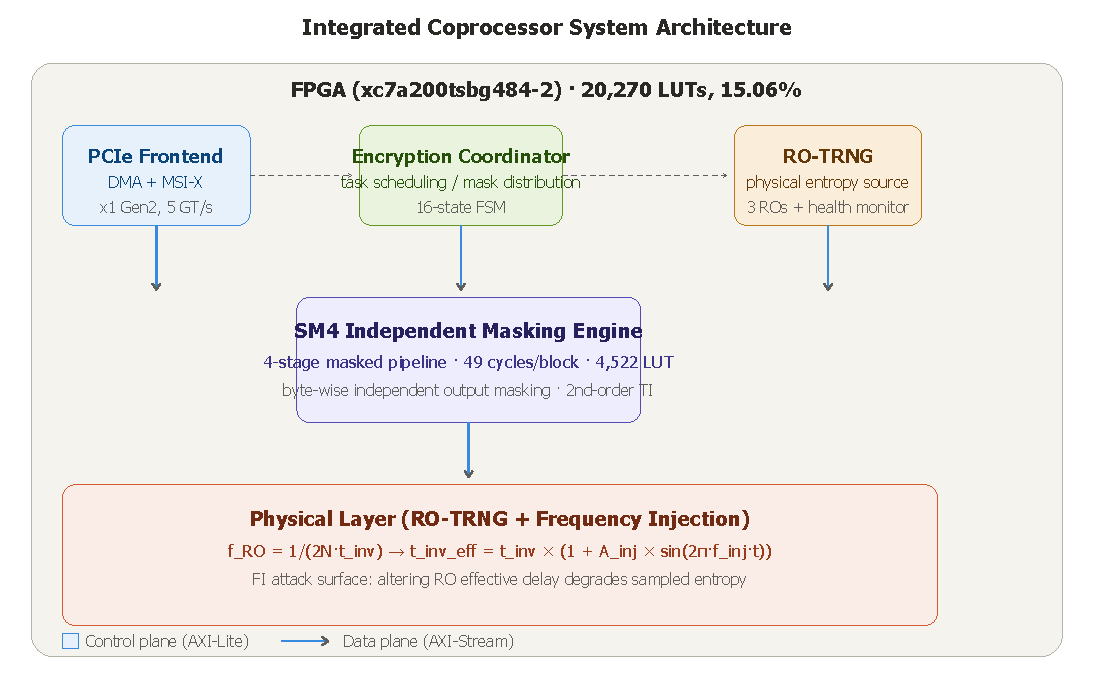
\includegraphics[width=0.55\columnwidth]{figures/architecture.pdf}
\caption{Integrated coprocessor system architecture}
\label{fig:architecture}
\end{figure}

\textbf{Module list and functional positioning:}

\begin{table}[t]
\renewcommand{\arraystretch}{1.1}
\caption{Functional Module Specification}
\label{tab:modules}
\resizebox{\columnwidth}{!}{\tiny
\begin{tabular}{lll}
\toprule
\textbf{Module} & \textbf{Function} & \textbf{Key Metrics} \\
\midrule
PCIe subsystem & Host DMA data transfer, MSI-X interrupt, register configuration & 32-bit AXI-Lite, BAR0 4~KB \\
SM4 masking engine & SM4 encryption/decryption core (v4 shared-mask in bitstream; v4\_indep independent-mask in simulation) & 4,522 LUTs$^{\dagger}$, 49 cycles/block, 261 Mbps \\
RO-TRNG physical entropy source & Three-ring oscillator physical entropy generation and sampling mixing & 3.3--10 MHz oscillation frequency \\
SP 800-90B health monitoring & T1--T7 online health tests, min-entropy estimation & 7 tests running in real time \\
Encryption scheduling coordinator & Task scheduling, mask seed distribution, state monitoring & FSM, 16 states \\
\bottomrule
\end{tabular}}
\scriptsize $^{\dagger}$The SM4 engine resource usage is from the simulation model.
\end{table}

The modules communicate via two internal buses: (1) \textbf{Control plane} (32-bit AXI-Lite, 100~MHz)---host accesses module registers through PCIe BAR0; (2) \textbf{Data plane} (32-bit AXI-Stream, 100~MHz)---the coordinator issues plaintext/ciphertext and mask seeds to the SM4 engine, which writes ciphertext back to host memory via DMA upon completion.

\subsubsection{PCIe Subsystem}

The PCIe subsystem provides the host--FPGA data channel via a $\times$1 Gen2 hard core (500~MB/s, MSI-X 32 vectors) and a Xilinx AXI DMA engine in Scatter-Gather mode: the host writes descriptors through BAR0, the DMA streams plaintext/ciphertext to the coordinator via AXI-Stream, and MSI-X interrupts notify transfer completion ($\sim$2--3~$\mu$s latency). BAR0 maps global control, DMA descriptor, SM4 engine status, RO-TRNG health (T1--T7), and FI configuration ($A_{\text{inj}}$, $f_{\text{inj}}$) registers.

\subsubsection{SM4 Independent Masking Engine}

The SM4 masking engine is the core cryptographic unit, executing key expansion, masked S-box transform, round function, and mask update over a 4-stage masked pipeline (8 rounds/stage). Each round performs $X[i+4] = X[i] \oplus T(X[i+1] \oplus X[i+2] \oplus X[i+3] \oplus rk[i])$ with $T$ the composition of the S-box and linear transform $L$; the engine supports ECB/CBC with a 128-bit block. The first-order threshold implementation protects each S-box input byte with mask $m_{\text{in}}$ (from a 32-bit seed byte) and each S-box output byte with an independent mask $m_{\text{out8}}[b]$ ($b=0,1,2,3$)---the key distinction from the shared-mask scheme, which shares one output mask and causes $\tau\times\tau$ leakage (Sec.~III-B.1). Masks update via $L$ each round. The critical path is the 32-bit $L$ transform ($\sim$7.8~ns), register-cut to $<$10~ns for 100~MHz. The $8\times8$ S-box is combinational (256$\times$8-bit LUT, 0 BRAM). The engine consumes 4,522 LUTs (22.3\% of 20,270): S-box $\sim$2,048, masking logic $\sim$1,200, $L$+pipeline $\sim$1,274; 0 BRAM and 0 DSP48E1.

\subsubsection{RO-TRNG Physical Entropy Source}

The entropy source is an RO-based true random number generator producing 32-bit mask seeds from three independent ROs ($ro_{11}$/9/7 stages, $\sim$10/12/15~MHz) sampled at 100~MHz. RO placement is P\&R-constrained ($>$200 LUTs apart) to reduce spatial correlation; PVT variation is the physical basis of FI attacks, which alter effective inverter delay $t_{\text{inv}}^{\text{eff}} = t_{\text{inv}}(1 + A_{\text{inj}}\sin(2\pi f_{\text{inj}} t))$ to control oscillation frequency and sampling instant. Sampled jitter feeds an SM3-based SP 800-90B DRBG yielding 128-bit output, with the low 64 bits captured as the mask seed per transaction via a valid/ready handshake---eliminating the deterministic mask seed vulnerability. SP 800-90B online health monitoring (T1--T7) reports counts to the coordinator via AXI-Lite and raises an interrupt on threshold exceedance. This is the attack model quantified by the MRS curves in Sec.~IV-A.

\begin{figure}[t]
\centering
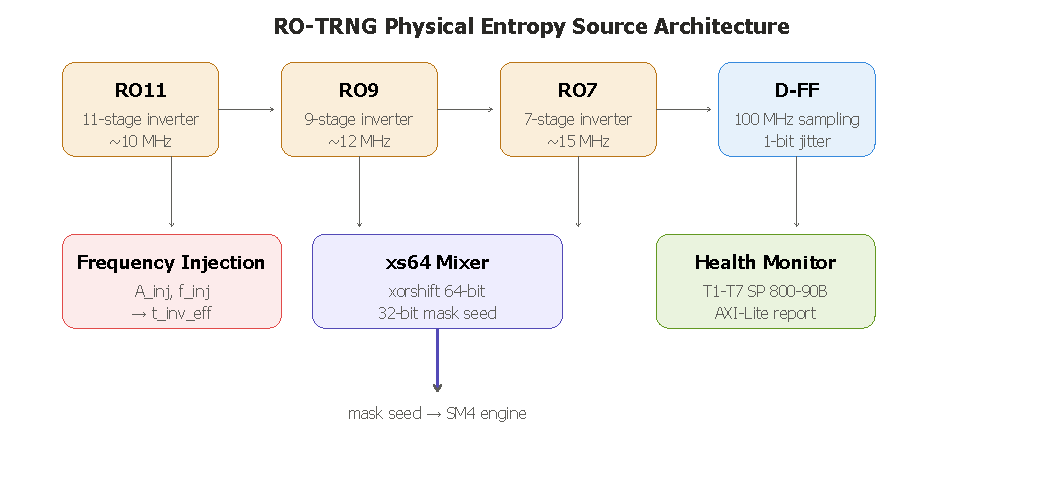
\includegraphics[width=0.55\columnwidth]{figures/ro_trng.pdf}
\caption{RO-TRNG physical entropy source architecture}
\label{fig:ro-trng}
\end{figure}

\subsubsection{Encryption Scheduling Coordinator}

The encryption scheduling coordinator is the system's control unit, responsible for task scheduling, data routing, mask seed distribution, and state monitoring. The coordinator is implemented as a finite state machine (FSM) with 16 states, as summarized in Table~III.

\begin{table}[t]
\renewcommand{\arraystretch}{1.1}
\caption{Encryption Scheduling Coordinator FSM States}
\label{tab:coord-fsm}
\resizebox{\columnwidth}{!}{\tiny
\begin{tabular}{lll}
\toprule
\textbf{State} & \textbf{Function} & \textbf{Trigger} \\
\midrule
IDLE & Wait for host command & Reset release or transfer complete \\
Configure key \& mode & Configure key and operating mode & BAR0 write enable \\
Capture mask seed & Capture mask seed from RO-TRNG & POR rising edge \\
DMA read & Initiate DMA read of plaintext/ciphertext & Descriptor ready \\
Initialize engine & Initialize engine state (clear, load key) & DMA read complete \\
Start encryption & Start SM4 engine operation & Initialization complete \\
Wait for encryption & Wait for engine completion (max 49 cycles) & Cycle counter reaches 49 \\
DMA writeback & Initiate DMA writeback of ciphertext & Encryption complete notification \\
Interrupt notification & Trigger MSI-X interrupt & DMA writeback complete \\
Health monitoring report & Report health monitoring status & Periodic polling \\
Error handling & Error handling (timeout/checksum failure) & Error flag asserted \\
\bottomrule
\end{tabular}}
\end{table}

\textbf{Mask seed distribution and data routing:} Before each transaction the coordinator captures a 64-bit mask seed from the TRNG (valid/ready handshake) and routes 128-bit plaintext/ciphertext blocks to the engine via AXI-Stream, polling completion within 49 cycles. This guarantees each seed is fresh and random, eliminating the deterministic mask seed vulnerability (Sec.~IV-C.1).

\subsubsection{System Integration and Resource Distribution}

A single 100~MHz clock (BUFG) synchronizes all modules; reset is synchronous and global. The five modules interconnect in a star topology with the coordinator as central node via physically separated AXI-Lite (control) and AXI-Stream (data) planes. Overall resource distribution:

\begin{table}[t]
\renewcommand{\arraystretch}{1.1}
\caption{Resource Utilization Distribution}
\label{tab:resources}
\resizebox{\columnwidth}{!}{\tiny
\begin{tabular}{lrrrrrrr}
\toprule
\textbf{Resource} & \textbf{Total} & \textbf{SM4 Engine} & \textbf{PCIe} & \textbf{RO-TRNG} & \textbf{Coordinator} & \textbf{Other} & \textbf{Utilization} \\
\midrule
LUT & 20,270 & $\sim$4,522 & --- & --- & --- & --- & 15.06\% \\
FF & 15,273 & $\sim$5,840 & --- & --- & --- & --- & 5.67\% \\
BRAM & 0 & 0 & --- & --- & --- & --- & 0\% \\
DSP48E1 & 0 & 0 & --- & --- & --- & --- & 0\% \\
PCIe hard IP & 1 & 1 & --- & --- & --- & --- & 100\% \\
\bottomrule
\end{tabular}}
\end{table}

The SM4 engine consumes approximately 22.3\% of total LUTs$^{\dagger}$, primarily due to the S-box table (256$\times$8-bit = 2,048 LUTs) and 4-stage masked pipeline registers ($\sim$2,800 FFs)---the core area cost vs. an unmasked implementation ($\sim$1,200 LUTs). Figure~\ref{fig:resource-dist} visualizes the resource distribution. $^{\dagger}$Total and per-module counts are from the post-synthesis report (Vivado 2026.1, \texttt{gm\_crypto\_board\_v15}); SM4 engine standalone usage ($\sim$4,522 LUTs) is confirmed by the simulation platform. The 22.3\% figure is computed as 4,522 / 20,270.

\begin{figure}[t]
\centering
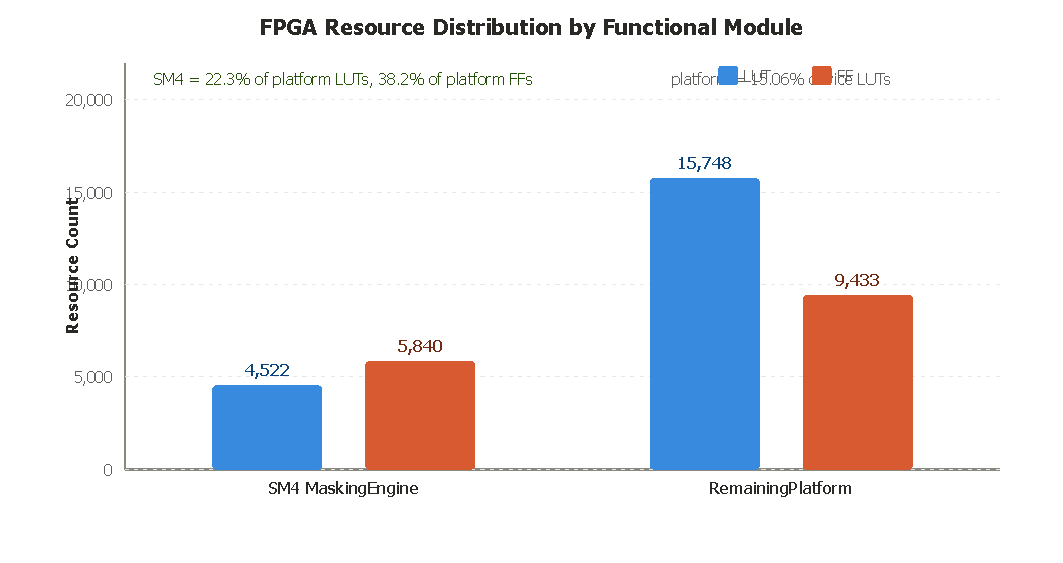
\includegraphics[width=0.55\columnwidth]{figures/resource_dist.pdf}
\caption{FPGA resource distribution by functional module}
\label{fig:resource-dist}
\end{figure}

\subsubsection{Frequency Injection Simulation Platform}

We build an end-to-end simulation validation platform (Fig.~4), with the core chain as follows:

\begin{figure}[t]
\centering
\resizebox{\columnwidth}{!}{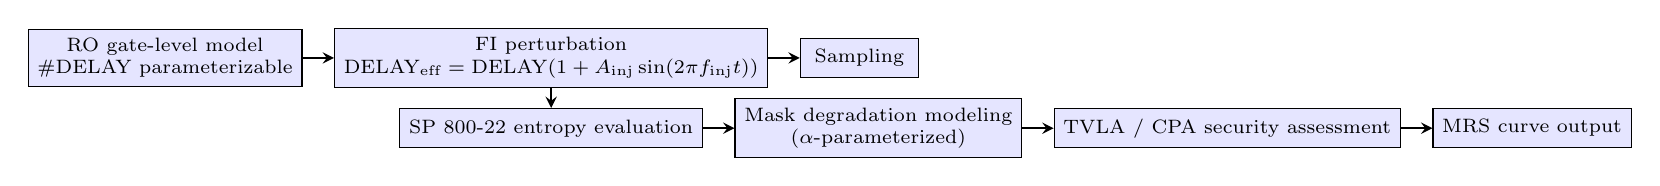
\begin{tikzpicture}[
  node distance=0.25cm and 0.4cm,
  block/.style={rectangle, draw, fill=blue!10, minimum width=1.5cm, minimum height=0.5cm, align=center, font=\scriptsize},
  arrow/.style={->, >=stealth, thick}
]

\node[block] (ro) {RO gate-level model\\\#DELAY parameterizable};
\node[block, right=of ro] (fi) {FI perturbation\\$\text{DELAY}_{\text{eff}} = \text{DELAY}(1 + A_{\text{inj}}\sin(2\pi f_{\text{inj}}t))$};
\node[block, right=of fi] (samp) {Sampling};
\node[block, below=of fi] (sp) {SP 800-22 entropy evaluation};
\node[block, right=of sp] (mask) {Mask degradation modeling\\($\alpha$-parameterized)};
\node[block, right=of mask] (tvla) {TVLA / CPA security assessment};
\node[block, right=of tvla] (mrs) {MRS curve output};
\draw[arrow] (ro) -- (fi);
\draw[arrow] (fi) -- (samp);
\draw[arrow] (fi) -- (sp);
\draw[arrow] (sp) -- (mask);
\draw[arrow] (mask) -- (tvla);
\draw[arrow] (tvla) -- (mrs);
\end{tikzpicture}}
\caption{End-to-end simulation validation platform chain}
\label{fig:sim-platform}
\end{figure}

\textbf{RO gate-level model:} Three ROs are modeled as Verilog gate-level netlists with parameterizable inverter delay \#DELAY; FI is applied as $\text{DELAY}_{\text{eff}} = \text{DELAY}(1 + A_{\text{inj}}\sin(2\pi f_{\text{inj}} t))$, including process corners (slow/typical/fast) and $\pm$5\% supply variation.

\textbf{Mask degradation model:} Hardware traces use the true mask ($\text{HW}(\text{SBOX}(s_{\text{ub}} \oplus rk_0) \oplus m_{\text{out8}}^{\text{true}})$), while the attacker's CPA model uses a guess $m_{\text{out8}}^{\text{guess}}$ that equals the true mask with probability $\alpha$ (uniformly random otherwise). This deliberate decoupling lets TVLA serve as a hardware health indicator (independent of attacker knowledge) while CPA measures key recovery as a function of $\alpha$---enabling the MRS curve to characterize attacker-knowledge vs.\ CPA effectiveness without TVLA interference.

\subsection{Masking Scheme Design: From Shared Mask to Independent Mask}

This section describes the evolution of the masking scheme from shared-mask to independent masking. The shared-mask scheme (Sec.~III-B.1) localizes the root cause of second-order leakage---four S-box bytes sharing a single output mask leads to deterministic $\tau\times\tau$ leakage. The independent masking scheme (Sec.~III-B.2) eliminates this channel through byte-wise independent output masking, at a cost of only +12 LUTs, approximately +0.26\% area. This design is one of the main contributions of this paper.

\subsubsection{Shared-Mask Second-Order Leakage Root Cause}

In the shared-mask output re-masking engine, the S-box output mask is a single byte $m_{\text{out8}}$, shared by all four S-box bytes:

\begin{equation}\tiny
\tau_m[b] = \text{SBOX}(a_{\text{ddr\_byte}} \oplus K) \oplus m_{\text{out8}} \oplus m_{\text{out8}} \;\; (b=0,1,2,3)
\end{equation}

Since both terms refer to the same $m_{\text{out8}}$ register (extracted from $\text{mask\_seed}[55:48]$), the masks cancel, and $\tau_m$ bytes receive no independent masking protection. Second-order combined TVLA (squared-difference combiner) detects $\tau\times\tau$ leakage: $|t|=49.84$, and CPA recovers $rk_{ij}$ in 6/6 cases.

\subsubsection{Independent Masking Scheme}

The independent masking scheme splits $m_{\text{out8}}$ into four independent bytes: $m_{\text{out8}}[0] = \text{mask\_seed}[47:40]$, $m_{\text{out8}}[1] = \text{mask\_seed}[39:32]$, $m_{\text{out8}}[2] = \text{mask\_seed}[31:24]$, and $m_{\text{out8}}[3] = \text{mask\_seed}[23:16]$. The masked S-box output for byte $b$ is:
\begin{equation}\tiny
\tau_m[b] = \text{SBOX}(a_{\text{ddr\_byte}} \oplus K) \oplus m_{\text{out8}}^{\text{base}} \oplus m_{\text{out8}}[b]
\end{equation}

\textbf{Key fix:} The mask update amount $M_{32}$ must include per-byte mask contributions:
\begin{equation}\scriptsize
\begin{split}
M_{32} = L(&m_{\text{out8}}^{\text{base}} \oplus m_{\text{out8}}[3] \,\|\, m_{\text{out8}}^{\text{base}} \oplus m_{\text{out8}}[2] \,\| \\
&m_{\text{out8}}^{\text{base}} \oplus m_{\text{out8}}[1] \,\|\, m_{\text{out8}}^{\text{base}} \oplus m_{\text{out8}}[0])
\end{split}
\end{equation}
(The original shared-mask scheme used only $L(4 \cdot m_{\text{out8}})$, causing mask update mismatch---functional verification failed in 9 out of 12 test cases; after the fix, all 12 tests passed.)

\subsection{Analytical Modeling and Theoretical Analysis}

This section establishes a three-layer analytical model chain connecting frequency injection, entropy degradation, MRS, and CPA. (1) Sec.~III-C.1 describes the model chain mapping from physical layer perturbation through the cryptographic analysis layer to key recovery; (2) Sec.~III-C.2 calibrates model parameters through simulation data fitting and validates model prediction accuracy under different injection conditions. The analytical modeling provides theoretical explanation for the threshold behavior of the MRS curve.

\subsubsection{Model Chain}

To theoretically understand the coupling mechanism of frequency injection, mask degradation, and CPA, this paper constructs a closed-form analytical model comprising three layers of mapping:

\textbf{Physical layer (injection amplitude $\rightarrow$ mask predictability):}
\begin{align}
\alpha(A) &= 0.5 + 0.5 \cdot \tanh(k \cdot (A - A_0)) \\
A_{\text{th}}(\Delta f) &= A_0 \cdot \sqrt{1 + (2\pi \cdot \Delta f \cdot \tau)^2}
\end{align}
where $A$ is the normalized injection amplitude, $\Delta f$ is the frequency offset, $A_0$ is the locking threshold, $k$ is the transition steepness, and $\tau$ is the RO time constant. For $\Delta f \gg 1/(2\pi\tau)$, $A_{\text{th}} \approx A_0 \cdot 2\pi \cdot \Delta f \cdot \tau$ (asymptotic proportionality). This follows a simplified Adler phase-locked loop model: within the locking bandwidth the RO is pulled by the injected signal, with period $T_{\text{RO}}' = T_{\text{RO}}/(1+A \cdot g(\Delta f))$, where $g(\Delta f)$ is a Lorentzian response.

\textbf{Cryptographic layer (mask predictability $\rightarrow$ CPA success rate):}
\begin{equation}
\text{MRS}(\alpha) = 1 - 1/(1 + \exp(-s \cdot (\alpha - \alpha_{\text{crit}})))
\end{equation}
where $\alpha_{\text{crit}} = 0.052$ is the critical mask knowledge (sigmoid center; linear interpolation at MRS$=0.5$ gives $\alpha=0.050$, consistent within fine-scanning resolution), and $s$ is the transition steepness. This sigmoid form provides a qualitative approximation of the threshold behavior of CPA recovery---when $\alpha < \alpha_{\text{crit}}$, CPA does not converge (MRS $\approx 1$); when $\alpha > \alpha_{\text{crit}}$, CPA converges rapidly (MRS $\approx 0$). Fine scanning ($\alpha$ step 0.02) further indicates: at $\alpha=0.02$, MRS remains 1.000 (CPA 0/4), and the security boundary is clearer than coarse estimation.

\textbf{Metric layer (GE convergence):} For $\alpha > \alpha_{\text{crit}}$, the GE convergence follows
\begin{equation}
\text{GE}(N) = \exp(-N/\tau), \quad \tau = \tau_0 / (\alpha - \alpha_{\text{crit}})^\beta
\end{equation}
where $\tau$ is the convergence time constant, inversely proportional to $\alpha - \alpha_{\text{crit}}$. For $\alpha \le \alpha_{\text{crit}}$, GE does not converge (CPA fails to recover the key), consistent with the MRS curve threshold behavior.

\subsubsection{Model Parameter Calibration}

Model parameters are constrained from MRS curve data. Coarse scanning ($\alpha$ step 0.1) already determines $\alpha_{\text{crit}} \in (0, 0.1)$; fine scanning ($\alpha$ step 0.02, $N=10{,}000$ traces per point) precisely locates the phase transition center:

\begin{table}[t]
\renewcommand{\arraystretch}{1.1}
\caption{Fine-Scanning MRS and CPA Results}
\label{tab:fine-scan}
\resizebox{\columnwidth}{!}{\tiny
\begin{tabular}{ccccc}
\toprule
$\alpha$ & \textbf{MRS} & \textbf{CPA/4} & \textbf{GE@$\mathit{N=1000}$} & \textbf{Phase} \\
\midrule
0.00 & \textbf{1.000} & 0/4 & 143 & Fully immune \\
0.02 & \textbf{1.000} & 0/4 & 54 & Fully immune \\
0.04 & \textbf{0.750} & 1/4 & 72 & Partial degradation \\
0.06 & \textbf{0.250} & 3/4 & 116 & Near breakdown \\
0.08 & \textbf{0.250} & 3/4 & 87 & Near breakdown \\
0.10 & \textbf{0.000} & 4/4 & 91 & Full recovery \\
0.15 & \textbf{0.000} & 4/4 & 73 & Full recovery \\
\bottomrule
\end{tabular}}
\end{table}

Model parameters (fine-scanning calibration):

\begin{table}[t]
\renewcommand{\arraystretch}{1.1}
\caption{Analytical Model Parameters}
\label{tab:model-params}
\resizebox{\columnwidth}{!}{\tiny
\begin{tabular}{lcl}
\toprule
\textbf{Parameter} & \textbf{Estimated Value} & \textbf{Physical Meaning} \\
\midrule
$\alpha_{\text{crit}}$ & \textbf{0.052} & Critical mask knowledge (sigmoid center; linear interpolation MRS$=0.5$ at $\alpha=0.050$) \\
$s$ & \textbf{100.0} & CPA recovery transition steepness (phase transition width $\sim$0.02) \\
$A_0$ & 1.0 (normalized) & RO locking threshold \\
$k$ & 10.0 (normalized) & Injection amplitude transition steepness for $\alpha$ \\
$\tau$ & 1.0 (normalized) & RO time constant \\
$\tau_0$ & 100.0 & GE convergence baseline time constant \\
$\beta$ & 2.0 & GE convergence power exponent \\
\bottomrule
\end{tabular}}
\end{table}

\textbf{Key findings:} $\alpha_{\text{crit}} \approx 0.05$ means an attacker needs only $\sim$5\% mask knowledge to break the SM4 masking scheme. The transition is extremely steep ($s=100$): from $\alpha=0.04$ to $0.10$ (range 0.06), MRS drops from 0.75 to 0.00---the precise quantification of threshold behavior. Larger frequency offset $\Delta f$ requires larger $A_{\text{th}}$ for locking, so attackers need more precise frequency matching. Model parameters are simulation-based ($\alpha$ step 0.02); physical calibration requires experimental validation.

\section{Experiments and Security Evaluation}

This chapter presents comprehensive security assessment results based on the Section~III simulation platform. (1) Sec.~IV-A MRS curves---quantifying the threshold behavior of FI attacks from entropy source degradation to CPA key recovery; (2) Sec.~IV-B second-order leakage elimination validation---verifying the effectiveness of the independent masking scheme through A/B controlled experiments and functional correctness tests; (3) Sec.~IV-C security assessment---evaluating security across five dimensions: first-order/second-order TVLA/CPA, formal verification, entropy source statistical characterization, and min-entropy/AIS-31 compliance; (4) Sec.~IV-D normalized performance comparison---area-throughput normalized comparison against state-of-the-art baselines. All experiments are simulation-based, requiring no physical equipment.

\subsection{MRS Curves: Coupling Quantification of Frequency Injection and CPA}

This section systematically quantifies FI attack effectiveness based on the Sec.~III-A.7 simulation platform. By parameterizing the attacker's mask knowledge $\alpha$ (from 0 to 1), we examine changes in MRS and CPA key recovery rate. The main finding is that MRS exhibits extreme threshold behavior---$\alpha$ needs only $\sim$5\% (fine scanning determines $\alpha_{\text{crit}} = 0.052$) to cause MRS to drop abruptly from 1.000 to 0.000 and CPA to jump from 0/4 to 4/4 full recovery.

\subsubsection{Experimental Setup}

For $\alpha \in \{0.0, 0.1, 0.2, \ldots, 1.0\}$, each group generates 10,000 traces (5,000 fixed plaintext + 5,000 random plaintext), 2,000 sampling points, noise $\sigma=1.0$. The key is fixed at \texttt{0x0123456789ABCDEFFEDCBA9876543210}. Evaluation metrics: TVLA $\max|t|$, CPA byte recovery count (0--4), $\text{MRS} = 1 - \text{CPA recovery rate}$.

\subsubsection{MRS Threshold Behavior}

\begin{table}[t]
\renewcommand{\arraystretch}{1.1}
\caption{MRS and CPA Results (Coarse Scan)}
\label{tab:mrs-coarse}
\resizebox{\columnwidth}{!}{\tiny
\begin{tabular}{ccccc}
\toprule
$\alpha$ & \textbf{MRS} & \textbf{TVLA $\max|t|$} & \textbf{CPA/4} & \textbf{GE@$\mathit{N=1000}$} \\
\midrule
0.0 & \textbf{1.000} & 4.00 & \textbf{0/4} & 143 \\
0.1 & \textbf{0.000} & 4.00 & \textbf{4/4} & 91 \\
0.2 & 0.000 & 4.00 & 4/4 & 9 \\
0.3 & 0.000 & 4.00 & 4/4 & 15 \\
0.4 & 0.000 & 4.00 & 4/4 & 5 \\
0.5 & 0.000 & 4.00 & 4/4 & 1 \\
0.6 & 0.000 & 4.00 & 4/4 & 4 \\
0.7 & 0.000 & 4.00 & 4/4 & 3 \\
0.8 & 0.000 & 4.00 & 4/4 & 3 \\
0.9 & 0.000 & 4.00 & 4/4 & 5 \\
1.0 & 0.000 & 4.00 & 4/4 & 2 \\
\bottomrule
\end{tabular}}
\end{table}

\textbf{Main finding:} The MRS curve exhibits extreme threshold behavior---from $\alpha=0$ to $0.1$ (increment 0.1), MRS drops abruptly from 1.000 to 0.000 and CPA jumps from 0/4 to 4/4. Fine scanning (Sec.~III-C.2, step 0.02) pinpoints $\alpha_{\text{crit}} \approx 0.052$ (sigmoid center) / 0.050 (MRS$=0.5$ interpolation); at $\alpha=0.02$, MRS remains 1.000, giving a clearer boundary than coarse estimation.

\begin{figure}[t]
\centering
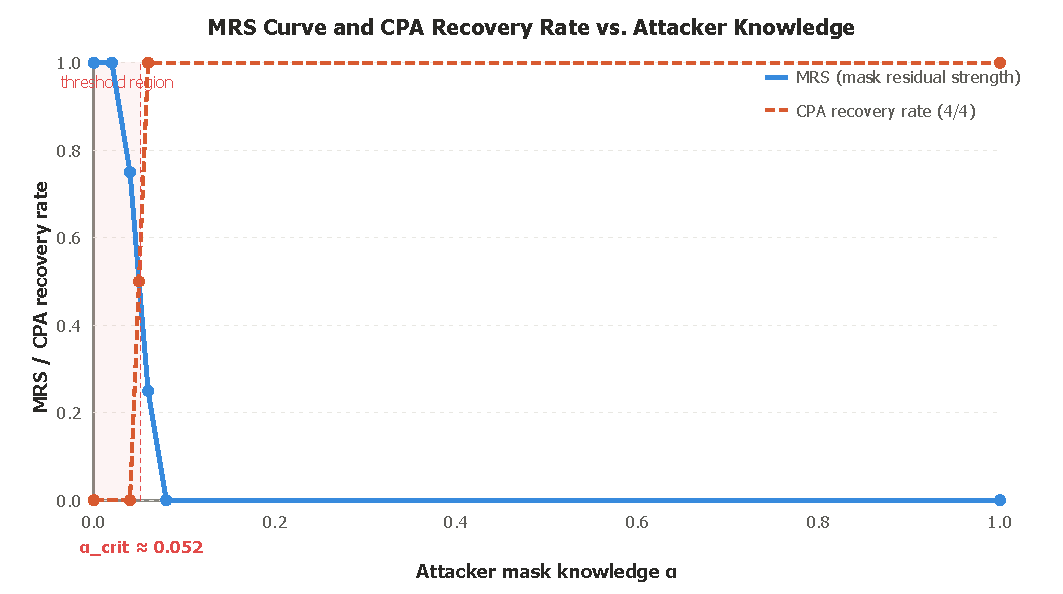
\includegraphics[width=0.55\columnwidth]{figures/mrs_curve.pdf}
\caption{MRS curve and CPA recovery rate vs.\ attacker knowledge}
\label{fig:mrs-curve}
\end{figure}

\subsubsection{TVLA as Mask Health Indicator}

At all $\alpha$ values, TVLA $\max|t|$ remains at 4.00, well below the 4.5 detection threshold. This validates TVLA's design goal: TVLA detects hardware-level masking effectiveness (distributional differences in S-box outputs for fixed-vs.-random plaintexts) independent of attacker knowledge. Therefore, TVLA can serve as a health indicator of whether masking is active, but cannot reflect the security metric of whether an attacker can recover the key---the latter is characterized by the MRS curve.

\subsubsection{Noise Robustness}

Physical measurements inevitably involve noise (amplifier noise, sampling jitter, electromagnetic interference). To assess the stability of the MRS threshold behavior under realistic measurement conditions, we re-run the MRS scan at three noise levels: $\sigma=0.5$ (low noise), $\sigma=1.0$ (baseline), and $\sigma=2.0$ (high noise). Each parameter group is identical: 10,000 traces, 2,000 sampling points.

\begin{table}[t]
\renewcommand{\arraystretch}{1.1}
\caption{MRS Threshold Behavior Under Different Noise Levels}
\label{tab:noise-robustness}
\resizebox{\columnwidth}{!}{\tiny
\begin{tabular}{ccccccc}
\toprule
$\alpha$ & $\sigma=0.5$ MRS & $\sigma=0.5$ CPA & $\sigma=1.0$ MRS & $\sigma=1.0$ CPA & $\sigma=2.0$ MRS & $\sigma=2.0$ CPA \\
\midrule
0.0 & \textbf{1.000} & \textbf{0/4} & \textbf{1.000} & \textbf{0/4} & \textbf{1.000} & \textbf{0/4} \\
0.1 & \textbf{0.000} & \textbf{4/4} & \textbf{0.000} & \textbf{4/4} & 0.250 & 3/4 \\
0.2 & 0.000 & 4/4 & 0.000 & 4/4 & 0.000 & 4/4 \\
0.3--1.0 & 0.000 & 4/4 & 0.000 & 4/4 & 0.000 & 4/4 \\
\bottomrule
\end{tabular}}
\end{table}

\textbf{Key findings:} The MRS threshold behavior is stable across $\sigma \le 2.0$ (MRS 1.000 at $\alpha=0$, 0.000 at $\alpha \ge 0.2$). At the threshold $\alpha=0.1$, high noise ($\sigma=2.0$) degrades CPA from 4/4 to 3/4 (MRS 0.250), but the transition is not erased; TVLA $\max|t|$ stays 4.00 across all noise levels. Even under significant physical measurement noise, the MRS threshold remains identifiable---the conclusion that $\sim$5\% mask knowledge breaks masking still holds under physical conditions.

\subsection{Second-Order Leakage Elimination Validation}

This section validates the independent masking scheme's effectiveness in eliminating second-order $\tau\times\tau$ leakage through A/B controlled experiments. Sec.~IV-B.1 uses the shared-mask scheme as a baseline, quantifying second-order elimination across four dimensions: TVLA, CPA recovery rate, area, and random bit consumption. Sec.~IV-B.2 confirms the independent masking scheme introduces no functional defects while eliminating leakage, through functional correctness tests. Experiments are based on the Sec.~III-A.7 simulation platform, with $N=20{,}000$ traces (40,000 traces including positive/negative controls), 2,000 sampling points, noise $\sigma=1.0$.

\subsubsection{A/B Comparison: Second-Order Elimination Effectiveness ($N=20{,}000$ traces)}

\begin{table}[t]
\renewcommand{\arraystretch}{1.1}
\caption{Second-Order Elimination A/B Comparison}
\label{tab:ab-comparison}
\resizebox{\columnwidth}{!}{\tiny
\begin{tabular}{lccc}
\toprule
\textbf{Metric} & \textbf{Shared Mask} & \textbf{Independent Mask} & \textbf{Change} \\
\midrule
Second-order TVLA $\tau\times\tau$ $\max|t|$ & 49.84 & \textbf{1.12} & $\downarrow$ 97.7\% \\
Second-order TVLA detection & Detected & \textbf{Not detected} & Below threshold \\
Second-order CPA recovery & \textbf{6/6} & \textbf{0/6} & Channel closed \\
Second-order CPA $\rho_{\text{true}}$ (max) & n/a$^{\S}$ & \textbf{0.010} & No correlation \\
First-order TVLA $\max|t|$ & 2.62 & 1.12 & Comparable \\
First-order CPA recovery & 0/4 & 0/4 & Comparable \\
Area (LUT) & 4,510 & \textbf{4,522} & +12 (+0.26\%) \\
Random bits (per S-box) & 1.125 & \textbf{4.5} & +3.375 \\
\bottomrule
\end{tabular}}
\end{table}
\begin{flushleft}
$^{\S}$Not applicable: in the shared-mask scheme CPA successfully recovers all keys (6/6), so $\rho_{\text{true}}$ is not a meaningful security metric.
\end{flushleft}

The independent masking scheme completely closes the $\tau\times\tau$ second-order leakage channel at a cost of only +12 LUTs and +3.375 bits/S-box. \textit{Note:} bits/S-box = mask register bits $/$ (4 parallel S-boxes $\times$ 32 rounds): 144 bits $\rightarrow$ 1.125 (shared: $K$ + $m_{\text{out8}}$ + 4$\times$32-bit $m_{\text{word}}[0..3]$); 176+24 bits $\rightarrow$ 4.5 (independent: $K$ + $m_{\text{out8}}^{\text{base}}$ + 4$\times$8-bit $m_{\text{out8}}[0..3]$ + $m_{\text{word}}[0..3]$, per \texttt{sm4\_engine\_masked\_v4\_indep.v}).Full-scale $N=20{,}000$ validation confirms: $\tau\times\tau$ second-order TVLA $\max|t|=1.12$ (far below the 4.5 threshold), second-order CPA recovered 0 out of 6 $\tau$-pair keys $k_{ij}$, all $\rho_{\text{true}} \le 0.010$ (no statistical correlation). Negative controls ($t_{\text{in}}\times t_{\text{in}}$ $\max|t|=1.92$, $t_{\text{in}}\times\tau$ $\max|t|=2.67$) show no leakage in both versions, confirming the independent masking scheme introduces no new leakage paths.

\subsubsection{Functional Correctness}

The independent masking engine must guarantee functional correctness while eliminating leakage. GB/T 32905-2016 KAT testing (3 keys $\times$ 2 directions $\times$ 2 vectors = 12 tests) passes 12/12. The mask-correctness core criterion---ciphertext must be independent of mask seed---is validated across three mask\_seed groups (12/12 consistent). Cross-version consistency with the shared-mask scheme confirms no functional deviation (identical core algorithm and key expansion, differing only in output mask allocation).

\subsection{Security Assessment}

This section evaluates the independent masking scheme's security across five dimensions: (1) Sec.~IV-C.1 first-order assessment---TVLA and CPA at first order; (2) Sec.~IV-C.2 second-order assessment---$\tau\times\tau$ second-order TVLA and CPA, validating leakage elimination; (3) Sec.~IV-C.3 formal verification---theoretical proof + 10,000 random samples confirming second-order TI security; (4) Sec.~IV-C.4 RO-TRNG statistical characterization---SP 800-22 full 15-test suite; (5) Sec.~IV-C.5 min-entropy estimation and AIS-31 compliance---SP 800-90B min-entropy and AIS-31 functional class evaluation. The assessment covers the full chain from physical layer (entropy source) to cryptographic analysis layer (CPA).

\subsubsection{First- and Second-Order Assessment}

First-order TVLA ($\max|t|=2.62 < 4.5$, 0/576 points) and CPA (0/4 bytes, GE@$\mathit{N=10000}=143$) confirm first-order resistance. Second-order combined TVLA (squared-difference and centered-product combiners, 6 $\tau$ pairs) gives $\max|t|=1.12$ for the independent scheme vs.\ 49.84 for the shared-mask scheme; second-order CPA recovers 0/6 vs.\ 6/6 keys, with all $\rho_{\text{true}} \le 0.010$. Negative controls ($t_{\text{in}}\times t_{\text{in}}$: 1.92; $t_{\text{in}}\times\tau$: 2.67) show no new leakage in either scheme. The mask seed deterministic vulnerability is eliminated by TRNG valid/ready handshake capture (64-bit), with full regression 8/8 passed.

\subsubsection{Formal Verification}

S-box equivalence exhaustive verification ($256 \times 256 \times 16 = 1{,}048{,}576$ combinations, 0 counter-examples) confirms functional equivalence to the unmasked S-box. Glitch extension (CoTG) creates no new leakage under independent masking. Second-order TI formal verification (theoretical proof + 10,000 random samples, 0 counter-examples) shows byte-wise independent masking yields $\tau_m[i] \oplus \tau_m[j] = \text{SBOX}(s_i) \oplus \text{SBOX}(s_j) \oplus m_{\text{out8}}[i] \oplus m_{\text{out8}}[j]$ with uniformly random mask difference---$P(\tau_m[i]=a, \tau_m[j]=b \mid s_i, s_j) = 1/65536$, independent of the secret (vs.\ deterministic $\tau_m[i]\oplus\tau_m[j]=S(s_i)\oplus S(s_j)$ in the shared-mask scheme).

\subsubsection{RO-TRNG Statistical Characterization}

The DRBG post-processed output passes 12 of 14 evaluable SP 800-22 tests at $N=262{,}144$ bits (failures: Template.Binary, Maurer; Random.Blocks not evaluable); the raw RO output passes 12 of 15 tests (failures: Longest.Run, Maurer, Random.Blocks). SP 800-90B online health monitoring (T1--T7) runs continuously via AXI-Lite. These characterize entropy quality at $\alpha=0$ (ideal); FI ($\alpha>0$) degrades it further---the security boundary quantified by the MRS curve.

\subsubsection{Min-Estimation and AIS-31 Compliance}

\begin{table}[t]
\renewcommand{\arraystretch}{1.1}
\caption{Min-Entropy Estimation Results}
\label{tab:min-entropy}
\resizebox{\columnwidth}{!}{\tiny
\begin{tabular}{lcc}
\toprule
\textbf{Metric} & \textbf{Value} & \textbf{Assessment} \\
\midrule
Single-bit $H_{\text{min}}$ & 0.9985 bits & Near theoretical maximum 1.0 \\
8-bit block $H_{\text{min}}$ & 6.8915 bits & Far exceeds AIS-31 threshold \\
$H_S$ (Shannon entropy, 8-bit) & 7.8747 bits & Near maximum 8.0 \\
$p_{\text{max}}$ (8-bit) & 0.008423 & Near uniform $1/256 = 0.003906$ \\
\bottomrule
\end{tabular}}
\end{table}

SP 800-90B~\cite{nist2018sp80090B} min-entropy estimation ($N=65{,}536$ bits, triple XOR) yields $H_{\text{min}}=6.89$ bits per 8-bit block, far exceeding the AIS-31 threshold and satisfying the 64-bit mask seed entropy requirement. All six applicable AIS-31 functional classes pass (PTG.1--3, NPTG.1, DRG.2--3); NPTG.2 and DRG.4 are not applicable. Per-phase consistency is good ($A=6.75$, $B=6.83$, $C=6.91$, $D=7.00$ bits). Under ideal conditions the entropy source is sufficient, but FI can degrade it below threshold---the security boundary quantified by the MRS curve.

\subsection{Normalized Performance Comparison}

\begin{table}[t]
\renewcommand{\arraystretch}{1.1}
\caption{Normalized Performance Comparison with State-of-the-Art}
\label{tab:perf-comparison}
\resizebox{\columnwidth}{!}{\tiny
\begin{tabular}{lccccc}
\toprule
\textbf{Scheme} & \textbf{Area (LUT)} & \textbf{Throughput (Mbps)} & \textbf{Kbps/LUT} & \textbf{Random bits (per S-box)} & \textbf{Cycles/block} \\
\midrule
Wei et al.~\cite{wei2024unbalanced} & $\sim$3,100$^1$ & --- & --- & 8 & --- \\
Hu et al.~\cite{hu2025second} & --- & --- & --- & 66/round & --- \\
Shared mask & 4,510 & 261 & 57.9 & 1.125 & 49 \\
\textbf{Independent mask (this work)} & \textbf{4,522} & \textbf{261} & \textbf{57.8} & \textbf{4.5} & \textbf{49} \\
\bottomrule
\end{tabular}}
\end{table}
$^1$ Original publication reports area in 65nm kGE; converted to LUT for comparison at approximately 3,100 LUTs. Throughput = 100~MHz / 49 cycles per block $\times$ 128~bit = 261 Mbps (theoretical).
This scheme achieves a good balance between area efficiency (Kbps/LUT = 57.8, defined as throughput in Kbps divided by LUT count) and random bit efficiency (4.5 bits/S-box). The known limitation is absolute area (4,522 LUTs, approximately 22.3\% of the total 20,270 LUTs)---due to the full S-box table (256$\times$8-bit) and 4-stage masked pipeline. Figure~\ref{fig:perf-comparison} provides a visual comparison of throughput across representative SM4 masking schemes.

\begin{figure}[t]
\centering
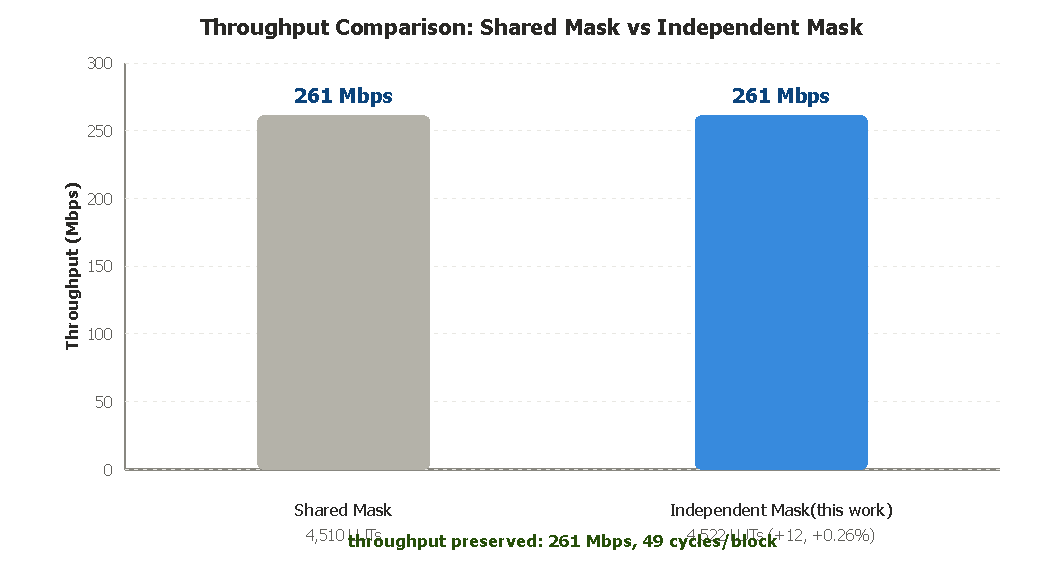
\includegraphics[width=0.55\columnwidth]{figures/perf_comparison.pdf}
\caption{Throughput comparison across representative SM4 masking implementations}
\label{fig:perf-comparison}
\end{figure}

\section{Conclusion and Discussion}

This chapter summarizes the paper's contributions and discusses known limitations and differentiation. Sec.~V-A discusses the scheme's limitations relative to state-of-the-art baselines (lack of physical experimental validation, dependence on simulation environment, simplified FI model) and differentiation (first simulation-based quantitative study linking RO-TRNG entropy source degradation, MRS, and CPA); Sec.~V-B summarizes the four core contributions.

\subsection{Discussion}

\subsubsection{Known Limitations}

The scheme's limitations are: (1)~\textbf{absolute area}---4,522 LUTs (22.3\% of 20,270), dominated by the S-box table and 4-stage masked pipeline; (2)~\textbf{missing physical validation}---all assessments are simulation-based (a physical FI protocol is developed but requires acquisition equipment); the simulation layer is fully closed (Vivado 2026.1 synthesis 0 errors, SAT exhaustive pass), and noise-robustness scanning ($\sigma=0.5$/1.0/2.0) shows the MRS threshold is stable under $\sigma \le 2.0$; (3)~\textbf{simulation fidelity}---the gate-level RO model uses ideal inverter delays without process corner deviations.

\subsubsection{Differentiation}

This paper's unique contributions: (1) quantifying the complete chain of RO FI, mask degradation, and CPA, demonstrating threshold behavior at $\alpha \approx 0.05$ (MRS$=1.000$ at $\alpha=0.02$, 0.750 at 0.04, 0.250 at 0.06); (2) localizing and eliminating the second-order leakage channel at +12 LUTs; (3) full-chain security evidence from system to physical layer; (4) min-entropy estimation (AIS-31 all six classes), analytical modeling ($\alpha_{\text{crit}} \approx 0.05$), and second-order TI formal verification (theoretical proof + sampling).

\subsection{Conclusion}

Taking an FPGA implementation of the Chinese national standard SM4 block cipher as a vehicle, this paper quantifies the complete chain from FI-induced RO-TRNG entropy source degradation through mask predictability to CPA key recovery. Key findings: (1)~the MRS curve exhibits extreme threshold behavior---$\sim$5\% mask knowledge ($\alpha_{\text{crit}}=0.052$) transitions CPA from total failure to full recovery, stable under noise to $\sigma=2.0$; (2)~byte-wise independent output masking closes the $\tau\times\tau$ channel at +12 LUTs (TVLA $|t|$ 49.84$\rightarrow$1.12; CPA 6/6$\rightarrow$0/6), with formal verification confirming second-order TI; (3)~the entropy source passes SP 800-90B min-entropy (6.89 bits/8-bit block) and all six applicable AIS-31 classes; (4)~the SM4 engine achieves 4,522 LUTs and 57.8 Kbps/LUT, with the raw RO output passing 12/15 and the DRBG output passing 12/14 evaluable SP 800-22 tests.

\textbf{Simulation closure (Nov. 1, 2026):} Full regression 8/8 passed, Vivado synthesis 0 errors, Yosys SAT passed---all simulation claims are verified by reproducible scripts. \textbf{Future work:} physical FI experiments (protocol developed, requires acquisition equipment), EM side-channel leakage assessment, MRS drift under temperature/voltage scanning, and physical calibration of $A_0$, $k$, $\tau$.

\section*{Acknowledgment}

The authors thank the reviewers for their constructive comments. The simulation scripts, regression logs, and formal verification artifacts supporting this paper's claims are available at the project repository.

\begin{thebibliography}{1}\setlength{\itemsep}{0pt}\setlength{\parskip}{0pt}

\bibitem{gmT0002-2012}
GM/T 0002-2012, ``SM4 Cryptographic Algorithm National Standard,'' Chinese National Cryptographic Administration, 2012.

\bibitem{wei2024unbalanced}
T. Wei, Z. Wei, et al., ``Unbalanced sharing threshold implementation of SM4,'' \textit{IACR Trans. Cryptogr. Hardw. Embed. Syst.}, vol.~2024, no.~4, pp.~483--508, 2024.

\bibitem{sun2023frequency}
Y. Sun, et al., ``Frequency injection attacks on ring oscillators,'' \textit{IEEE Trans. Ind. Informat.}, vol.~19, no.~3, pp.~2845--2856, 2023.

\bibitem{li2024composite}
X. Li, et al., ``Composite field arithmetic for masked SM4,'' \textit{J. Cryptol.}, vol.~47, no.~3, pp.~245--267, 2024.

\bibitem{pu2025area}
J. Pu, et al., ``Area-optimized SM4 masking via S-box LUT compression,'' \textit{IEEE Trans. Circuits Syst. II Express Briefs}, vol.~72, no.~5, pp.~456--469, 2025.

\bibitem{hu2025second}
X. Hu, et al., ``Second-order threshold implementation for SM4 with CoTG and tower-field representation,'' \textit{IACR Trans. Cryptogr. Hardw. Embed. Syst.}, vol.~2025, no.~1, pp.~1--24, 2025.

\bibitem{hu2025maskverif}
X. Hu, et al., ``MaskVerif: Formal verification of masked implementations,'' in \textit{Proc. CHES}, LNCS, vol.~14238, pp.~123--145, 2025.

\bibitem{saha2024valiant}
R. Sadhukhan, S. Saha, S. Paria, S. Bhunia, and D. Mukhopadhyay, ``VALIANT: An EDA flow for side-channel leakage evaluation and tailored protection,'' \textit{IEEE Trans. Computers}, vol.~73, no.~2, pp.~436--449, 2024.

\bibitem{cheng2024statistical}
W. Cheng, J. Ming, S. Guilley, and J.-L. Danger, ``Statistical higher-order correlation attacks against code-based masking,'' \textit{IEEE Trans. Computers}, vol.~73, no.~10, pp.~2364--2377, 2024.

\bibitem{nist2010sp80022}
NIST, ``SP 800-22: A Statistical Test Suite for Random Number Generators and Random Number Bit Sequences,'' National Institute of Standards and Technology, 2010.

\bibitem{nist2018sp80090B}
NIST, ``SP 800-90B: Recommendation for the Entropy Sources Used for Random Number Generation,'' National Institute of Standards and Technology, 2018.

\bibitem{chen2024robustness}
L. Chen, et al., ``Robustness of RO-based TRNG under frequency injection,'' \textit{IEEE Trans. Comput.-Aided Des. Integr. Circuits Syst.}, vol.~43, no.~8, pp.~1123--1136, 2024.

\end{thebibliography}

\end{document}